\documentclass[9pt,aspectratio=169,xcolor=table]{beamer}

%~~~~~~~~~~~~~~~~~~~~~~~~~~~~~~~~~~~~~~~~~~~~~~~~~~~~~~~~~~~~~~~~~~~~~~~~~~~~~~
% Use roboto Font (recommended)
\usepackage[sfdefault]{roboto}
\usepackage[utf8]{inputenc}
\usepackage[T1]{fontenc}
%~~~~~~~~~~~~~~~~~~~~~~~~~~~~~~~~~~~~~~~~~~~~~~~~~~~~~~~~~~~~~~~~~~~~~~~~~~~~~~

%~~~~~~~~~~~~~~~~~~~~~~~~~~~~~~~~~~~~~~~~~~~~~~~~~~~~~~~~~~~~~~~~~~~~~~~~~~~~~~
% Define where theme files are located. ('/styles')
\usepackage{styles/fluxmacros}
\usefolder{styles}
% Use Flux theme v0.1 beta
% Available style: asphalt, blue, red, green, gray
\usetheme[style=hunter]{flux}
%~~~~~~~~~~~~~~~~~~~~~~~~~~~~~~~~~~~~~~~~~~~~~~~~~~~~~~~~~~~~~~~~~~~~~~~~~~~~~~

%~~~~~~~~~~~~~~~~~~~~~~~~~~~~~~~~~~~~~~~~~~~~~~~~~~~~~~~~~~~~~~~~~~~~~~~~~~~~~~
% Extra packages
\usepackage{booktabs}
\usepackage{colortbl}
\usepackage{ragged2e}
\usepackage{amssymb}
\usepackage{multirow}
\usepackage{tikz}
\usetikzlibrary{arrows.meta, positioning, fit, backgrounds, calc, decorations.pathreplacing}
\setbeamertemplate{itemize items}[square]
\usepackage[scaled=.8]{beramono}
\usepackage{listings}
\usepackage{styles/lstlangarm}
\usepackage{array}
\definecolor{bgcolor}{HTML}{F2E9E9}
% lstlangarm.sty references \color{mauve} for string literals but never defines
% it -- only fires when a listing contains a string. Define it here.
\definecolor{mauve}{rgb}{0.58,0,0.82}
% lstlangarm's C style sets commentstyle=green!20, which is unreadable on the
% pink listing background. Darken it globally.
\lstset{commentstyle=\color{green!45!black}}
% ragged-right fixed-width column -- must be defined in the preamble, never
% inside a frame (\newcolumntype's #1 breaks beamer's frame scanner)
\newcolumntype{R}[1]{>{\RaggedRight\arraybackslash}p{#1}}
%~~~~~~~~~~~~~~~~~~~~~~~~~~~~~~~~~~~~~~~~~~~~~~~~~~~~~~~~~~~~~~~~~~~~~~~~~~~~~~
% Table striping: odd rows white, even rows very light gray.
% Needs \documentclass[...,xcolor=table]{beamer} (beamer loads xcolor itself,
% so the option must go on the class, not \usepackage).
\definecolor{stripe}{gray}{0.94}
% \striped makes body rows alternate white, gray, white, ... starting white.
% \rowcolors counts from the first coloured body row; the header is not counted.
\newcommand{\striped}{\rowcolors{1}{white}{stripe}}
%~~~~~~~~~~~~~~~~~~~~~~~~~~~~~~~~~~~~~~~~~~~~~~~~~~~~~~~~~~~~~~~~~~~~~~~~~~~~~~

%~~~~~~~~~~~~~~~~~~~~~~~~~~~~~~~~~~~~~~~~~~~~~~~~~~~~~~~~~~~~~~~~~~~~~~~~~~~~~~
% TikZ block styles -- matches ch1/ch2
% Colour variables are named identically in the book's stm32primer.tex, so any
% tikzpicture using only the \tikzset{...} styles below can be copied verbatim
% between slides and book. Only the \definecolor/\colorlet VALUES differ: the
% book is printed, so it keeps every stroke pure black with muted fills. These
% slides are projected, so both fill AND stroke are bright and saturated to
% grab attention -- see stm32primer.tex for the print palette.
\definecolor{blkfill}{HTML}{DDEEDD}
\definecolor{blkline}{HTML}{355E3B}
\definecolor{accentfill}{HTML}{FFE0B2}
\definecolor{accentline}{HTML}{E65100}
\definecolor{memfill}{HTML}{DFF5DA}
\definecolor{memline}{HTML}{2E7D32}
\definecolor{cellfill}{HTML}{FFFFFF}
\definecolor{cellline}{HTML}{424242}
\definecolor{bitmaskfill}{HTML}{DCEBFF}
\definecolor{bitmaskline}{HTML}{1565C0}
\definecolor{bithitfill}{HTML}{FFE0B2}
\definecolor{bithitline}{HTML}{E65100}
\tikzset{
  blk/.style   = {rectangle, rounded corners=2pt, draw=blkline, fill=blkfill,
                  thick, align=center, font=\small, minimum height=9mm, inner sep=3pt},
  cpublk/.style= {rectangle, rounded corners=2pt, draw=accentline, fill=accentfill,
                  thick, align=center, font=\small\bfseries, minimum height=9mm, inner sep=3pt},
  memblk/.style= {rectangle, rounded corners=2pt, draw=memline, fill=memfill,
                  thick, align=center, font=\small, minimum height=9mm, inner sep=3pt},
  cell/.style  = {rectangle, draw=cellline, fill=cellfill, align=center,
                  font=\small\ttfamily, minimum height=7mm, inner sep=2pt},
  bitcell/.style={rectangle, draw=cellline, fill=cellfill, thick,
                  minimum width=5.4mm, minimum height=5.4mm, inner sep=0pt,
                  font=\scriptsize\ttfamily, anchor=center},
  bitmask/.style={bitcell, fill=bitmaskfill, draw=bitmaskline},
  bithit/.style ={bitcell, fill=bithitfill, draw=bithitline, font=\scriptsize\ttfamily\bfseries},
  rowlab/.style ={font=\scriptsize, text=Gray, anchor=east},
  oplab/.style  ={font=\scriptsize\itshape, text=Gray, anchor=west},
  lbl/.style   = {font=\scriptsize, text=Gray},
  flow/.style  = {-{Stealth[length=2mm]}, thick, draw=blkline},
  busline/.style={thick, draw=cellline},
}
% NOTE (theme quirks -- all fail SILENTLY, always page through the PDF):
%  - a second \\ inside a nested {...} group in a TikZ node breaks parsing
%  - {\small ...} wrapped around a nested itemize eats the frame title + list
%  - \usebeamercolor on a [plain] frame falls through to an unstyled default
%  - \newcolumntype inside a frame breaks beamer's frame scanner
%  - lstlisting needs \begin{frame}[fragile]
%  - a TikZ picture wider than its column silently overflows into neighbours
%~~~~~~~~~~~~~~~~~~~~~~~~~~~~~~~~~~~~~~~~~~~~~~~~~~~~~~~~~~~~~~~~~~~~~~~~~~~~~~

%%%%%%%%%%%%%%%%%%%%%%%%%%%%%%%%%%%
%% BEGIN CONDITIONAL COMPILATION %%
%%%%%%%%%%%%%%%%%%%%%%%%%%%%%%%%%%%
\newif\ifwebex
%\webextrue % uncomment to generate section separator
\ifwebex
\AtBeginSection[]{
  \begin{frame}
  \vfill
  \centering
  \begin{beamercolorbox}[sep=8pt,center,shadow=true,rounded=true]{title}
    \usebeamerfont{title}\insertsectionhead\par%
  \end{beamercolorbox}
  \vfill
  \end{frame}
}
\else
\AtBeginSection[]
{
{
    \setbeamercolor{background canvas}{bg=yellow!10}
    \begin{frame}[plain]
        \frametitle{Table of Contents}
        \tableofcontents[currentsection]
    \end{frame}
}
}
\fi
%%%%%%%%%%%%%%%%%%%%%%%%%%%%%%%%%%%
%% END CONDITIONAL COMPILATION   %%
%%%%%%%%%%%%%%%%%%%%%%%%%%%%%%%%%%%

%~~~~~~~~~~~~~~~~~~~~~~~~~~~~~~~~~~~~~~~~~~~~~~~~~~~~~~~~~~~~~~~~~~~~~~~~~~~~~~
% Information
\title{Number Systems I}
\subtitle{\emph{Contemporary Digital Electronic Systems} --- Chapter 2}
\author{Mun\'{i}m Zabidi}
\institute{\color{primary}Faculty of Electrical Engineering, Universiti Teknologi Malaysia}
\date{\today}
\titlegraphic{assets/logoutmwhite.png}
\graphicspath{{.}{../fig/}}
%~~~~~~~~~~~~~~~~~~~~~~~~~~~~~~~~~~~~~~~~~~~~~~~~~~~~~~~~~~~~~~~~~~~~~~~~~~~~~~

\begin{document}

\titlepage

%===============================================================================
\section{Why This Chapter}
%===============================================================================

\begin{frame}{Why This Chapter Matters}
  \begin{columns}[c]
  \begin{column}{.47\textwidth}
    Every value a digital circuit stores, computes or transmits is a \alert{pattern of bits}. Reading, writing and converting between number systems, and recognising the common binary codes, is the foundational literacy for everything that follows.
  \end{column}
  \begin{column}{.51\textwidth}
    \begin{block}{After this chapter, you can:}
    {\small
    \begin{enumerate}\itemsep2pt
      \item Convert integers and fractions between decimal, binary, octal and hexadecimal.
      \item Count in each system and recognise place values.
      \item Encode a decimal digit in BCD and read it back.
      \item Explain why Gray code changes one bit at a time.
      \item Encode characters in ASCII; know how Unicode differs.
    \end{enumerate}}
    \end{block}
  \end{column}
  \end{columns}
\end{frame}

\begin{frame}{An Opening Question}
  \leavevmode\vspace{4mm}
  The decimal number 1000 fits in four digits.
  \vspace{4mm}
  \begin{center}
  \fbox{\parbox{.78\textwidth}{\centering\vspace{2mm}
  \large How many \alert{bits} are needed to store the same value in binary, and how many \alert{hexadecimal} digits?
  \vspace{2mm}}}
  \end{center}
  \vspace{4mm}
  By the end of the chapter you should answer without a calculator.
\end{frame}

%===============================================================================
\section{Decimal and Binary}
%===============================================================================

\begin{frame}{Positional Notation}
  \begin{itemize}
    \item The number of symbols in a counting system is its \alert{base} or \alert{radix}. Decimal has radix 10; digital systems use radix 2.
    \item A digit's value depends on its \alert{position}. For 786.3:
  \end{itemize}
  \begin{center}
  \begin{tabular}{|c|c|c|c|c|}
    \hline
    7 & 8 & 6 & . & 3 \\ \hline
    $10^{2}$ & $10^{1}$ & $10^{0}$ & . & $10^{-1}$ \\ \hline
  \end{tabular}
  \end{center}
  \begin{block}{Any base $b$}
    \[ N_b = a_{n-1}b^{n-1} + \cdots + a_1 b^1 + a_0 b^0 + a_{-1}b^{-1} + \cdots + a_{-m}b^{-m} \]
  \end{block}
\end{frame}

\begin{frame}{Binary Numbers}
  \begin{columns}[t]
  \begin{column}{.5\textwidth}
    \begin{itemize}\small
      \item Each digit is a \alert{bit}: 0 or 1.
      \item Leftmost bit: \alert{MSB} (most significant). Rightmost: \alert{LSB}.
      \item Weights are powers of two.
    \end{itemize}
    \vspace{2mm}
    \begin{center}
    \begin{tabular}{|c|c|c|c|c|c|c|c|}
      \hline
      $2^7$ & $2^6$ & $2^5$ & $2^4$ & $2^3$ & $2^2$ & $2^1$ & $2^0$ \\ \hline
      128 & 64 & 32 & 16 & 8 & 4 & 2 & 1 \\ \hline
    \end{tabular}
    \end{center}
  \end{column}
  \begin{column}{.46\textwidth}
    \centering\footnotesize\striped
    \begin{tabular}{@{}crl@{}}
      \toprule
      $n$ & $2^n$ & $2^{-n}$ \\
      \midrule
      0 & 1 & 1 \\
      1 & 2 & 0.5 \\
      2 & 4 & 0.25 \\
      3 & 8 & 0.125 \\
      4 & 16 & 0.0625 \\
      5 & 32 & 0.03125 \\
      \bottomrule
    \end{tabular}
  \end{column}
  \end{columns}
\end{frame}

\begin{frame}{Binary to Decimal}
  Add the weights of the bits that are 1; ignore the 0s.
  \begin{block}{Example: $1011011_2$}
    \centering\small
    \begin{tabular}{l|c|c|c|c|c|c|c|}
      \cline{2-8}
      Weights: & $2^6$ & $2^5$ & $2^4$ & $2^3$ & $2^2$ & $2^1$ & $2^0$ \\ \cline{2-8}
      Bits: & 1 & 0 & 1 & 1 & 0 & 1 & 1 \\ \cline{2-8}
    \end{tabular}
    \[ 1011011_2 = 64 + 16 + 8 + 2 + 1 = 91_{10} \]
  \end{block}
  \begin{block}{Example: $1.01_2$}
    \[ 1.01_2 = 2^0 + 2^{-2} = 1 + \tfrac14 = 1.25_{10} \]
  \end{block}
\end{frame}

\begin{frame}{Decimal to Binary: Sum of Weights}
  Subtract the greatest power of two that fits; repeat until nothing is left.
  \begin{block}{Example: $19_{10}$}
    \begin{enumerate}\small\itemsep1pt
      \item Biggest power of 2 below 19 is 16: $19 - 16 = 3$.
      \item $3 - 2 = 1$.
      \item $1 - 1 = 0$.
      \item So $19 = 16 + 2 + 1$.
    \end{enumerate}
    \centering
    \begin{tabular}{|c|c|c|c|c|}
      \hline
      16 & 8 & 4 & 2 & 1 \\ \hline
      1 & 0 & 0 & 1 & 1 \\ \hline
    \end{tabular}
    \quad $\Rightarrow\ 19_{10} = 10011_2$
  \end{block}
\end{frame}

\begin{frame}{Decimal to Binary: Repeated Division}
  \begin{columns}[c]
  \begin{column}{.38\textwidth}
    \centering
    \begin{tabular}{c|rc}
      \multicolumn{2}{c}{} & remainder \\
      37 & $\div2$ & 1 \\ \cline{1-2}
      18 & $\div2$ & 0 \\ \cline{1-2}
       9 & $\div2$ & 1 \\ \cline{1-2}
       4 & $\div2$ & 0 \\ \cline{1-2}
       2 & $\div2$ & 0 \\ \cline{1-2}
       1 & $\div2$ & 1 \\ \cline{1-2}
       0 & & (stop) \\
    \end{tabular}
  \end{column}
  \begin{column}{.58\textwidth}
    \begin{itemize}
      \item Divide by 2, record the remainder, repeat with the quotient until it is 0.
      \item The \alert{first} remainder is the LSB; read upwards.
      \item $37_{10} = 100101_2$.
      \item Check: $32 + 4 + 1 = 37$.
    \end{itemize}
  \end{column}
  \end{columns}
\end{frame}

\begin{frame}{Decimal Fractions to Binary}
  Integer part by repeated division; fraction part by repeated \alert{multiplication} by 2.
  \begin{block}{Example: $2.25_{10}$}
    \small
    Integer: $2 \div 2 = 1$ r 0 (LSB), $1 \div 2 = 0$ r 1 (MSB) $\Rightarrow 10_2$.

    \vspace{2mm}
    Fraction:
    \begin{center}
    \begin{tabular}{lcccl}
      0.25 & $\times$ & 2 & = & 0.5 \quad keep integer 0 \\
      0.5  & $\times$ & 2 & = & 1.0 \quad keep integer 1; fraction is 0, stop \\
    \end{tabular}
    \end{center}
    Fraction is $.01_2$, so $2.25_{10} = 10.01_2$.
  \end{block}
\end{frame}

%===============================================================================
\section{Bit Groups}
%===============================================================================

\begin{frame}{Common Bit Groups}
  \begin{columns}[t]
  \begin{column}{.4\textwidth}
    \centering\small\striped
    \begin{tabular}{@{}lc@{}}
      \toprule
      \textbf{Name} & \textbf{Bits} \\
      \midrule
      Bit & 1 \\
      Nibble & 4 \\
      Byte (octet) & 8 \\
      Word & 16, 32 or 64 \\
      \bottomrule
    \end{tabular}
  \end{column}
  \begin{column}{.58\textwidth}
    \begin{itemize}\small\itemsep2pt
      \item A \alert{word} is a system's native data size (32 bits on ARM).
      \item $n$ bits hold values up to $2^n - 1$.
      \item To store $x$ distinct values you need $\lceil \log_2 x \rceil$ bits.
    \end{itemize}
    \centering\footnotesize\striped
    \begin{tabular}{@{}cr@{}}
      \toprule
      $n$ & Largest value \\
      \midrule
      4 & 15 \\ 8 & 255 \\ 16 & 65\,535 \\ 32 & 4\,294\,967\,295 \\
      \bottomrule
    \end{tabular}
  \end{column}
  \end{columns}
\end{frame}

\begin{frame}{Storage and Speed Prefixes}
  \begin{columns}[t]
  \begin{column}{.42\textwidth}
    \centering\small\striped
    \begin{tabular}{@{}cccc@{}}
      \toprule
      \textbf{Prefix} & \textbf{Sym.} & $2^n$ & $10^n$ \\
      \midrule
      kilo & K & $2^{10}$ & $10^3$ \\
      mega & M & $2^{20}$ & $10^6$ \\
      giga & G & $2^{30}$ & $10^9$ \\
      tera & T & $2^{40}$ & $10^{12}$ \\
      \bottomrule
    \end{tabular}
  \end{column}
  \begin{column}{.56\textwidth}
    \begin{itemize}\small\itemsep2pt
      \item \alert{Storage}: powers of 2. 1\,KB = 1024 bytes.
      \item \alert{Everything else} (clock, power, data rate): powers of 10. 1\,Mbps = $10^6$ bit/s.
      \item 1\,MBps = 8\,000\,000 bit/s.
    \end{itemize}
  \end{column}
  \end{columns}
  \begin{block}{Example: addressing 8\,KB}
    \small $8 \times 1024 = 8192$ bytes, so $n = \lceil \log_2 8192 \rceil = 13$ address bits.
  \end{block}
\end{frame}

\begin{frame}{Expanding and Shrinking Binary Numbers}
  \begin{columns}[c]
  \begin{column}{.38\textwidth}
    \centering
    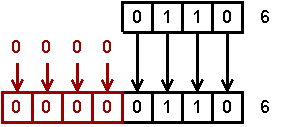
\includegraphics[width=\textwidth]{extend4t8_u}\\
    {\small Expand: pad 0s at the MSB end}
  \end{column}
  \begin{column}{.58\textwidth}
    \centering
    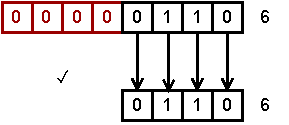
\includegraphics[width=.48\textwidth]{trunc_8t4_ok}\hfill
    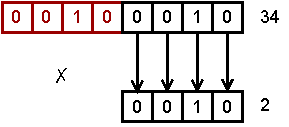
\includegraphics[width=.48\textwidth]{trunc_8t4_ko}\\
    {\small Shrink: OK only if every removed bit is 0}
  \end{column}
  \end{columns}
  \vspace{2mm}
  \begin{itemize}\small
    \item Truncation removes bits. If a removed upper bit is 1, the value changes.
  \end{itemize}
\end{frame}

%===============================================================================
\section{Octal and Hexadecimal}
%===============================================================================

\begin{frame}{Octal: Three Bits per Digit}
  \begin{columns}[t]
  \begin{column}{.5\textwidth}
    \begin{itemize}\small\itemsep2pt
      \item Symbols 0 to 7; each digit is exactly \alert{3 bits}.
      \item Conversion to and from binary is direct substitution.
    \end{itemize}
    \centering\footnotesize\striped
    \begin{tabular}{@{}cccccccc@{}}
      \toprule
      0 & 1 & 2 & 3 & 4 & 5 & 6 & 7 \\
      \midrule
      000 & 001 & 010 & 011 & 100 & 101 & 110 & 111 \\
      \bottomrule
    \end{tabular}
  \end{column}
  \begin{column}{.48\textwidth}
    \begin{block}{$1357_8$ to decimal}
      \small $1\!\times\!8^3 + 3\!\times\!8^2 + 5\!\times\!8^1 + 7\!\times\!8^0$\\
      $= 512 + 192 + 40 + 7 = 751_{10}$
    \end{block}
    \begin{block}{$2145_8$ to binary}
      \small 2 \ 1 \ 4 \ 5 $\to$ 010 \ 001 \ 100 \ 101\\
      $= 010001100101_2$
    \end{block}
  \end{column}
  \end{columns}
\end{frame}

\begin{frame}{Decimal to Octal; Binary to Octal}
  \begin{columns}[t]
  \begin{column}{.5\textwidth}
    \begin{block}{$2935_{10}$: repeated division by 8}
      \small
      \begin{tabular}{rcrcl}
        2935 & $\div 8$ & 366 & r & 7 (LSD) \\
        366 & $\div 8$ & 45 & r & 6 \\
        45 & $\div 8$ & 5 & r & 5 \\
        5 & $\div 8$ & 0 & r & 5 (MSD) \\
      \end{tabular}\\[1mm]
      $2935_{10} = 5567_8$
    \end{block}
  \end{column}
  \begin{column}{.48\textwidth}
    \begin{block}{$1101110010_2$ to octal}
      \small Group in threes from the right; pad the left with 0s:\\[1mm]
      \centering
      \begin{tabular}{cccc}
        001 & 101 & 110 & 010 \\
        1 & 5 & 6 & 2 \\
      \end{tabular}\\[1mm]
      $= 1562_8$
    \end{block}
  \end{column}
  \end{columns}
\end{frame}

\begin{frame}{Hexadecimal: Four Bits per Digit}
  \begin{columns}[c]
  \begin{column}{.42\textwidth}
    \centering\scriptsize\striped
    \begin{tabular}{@{}ccc|ccc@{}}
      \toprule
      Dec & Bin & Hex & Dec & Bin & Hex \\
      \midrule
      0 & 0000 & 0 & 8 & 1000 & 8 \\
      1 & 0001 & 1 & 9 & 1001 & 9 \\
      2 & 0010 & 2 & 10 & 1010 & A \\
      3 & 0011 & 3 & 11 & 1011 & B \\
      4 & 0100 & 4 & 12 & 1100 & C \\
      5 & 0101 & 5 & 13 & 1101 & D \\
      6 & 0110 & 6 & 14 & 1110 & E \\
      7 & 0111 & 7 & 15 & 1111 & F \\
      \bottomrule
    \end{tabular}
  \end{column}
  \begin{column}{.56\textwidth}
    \begin{itemize}\small\itemsep2pt
      \item 16 symbols: 0 to 9 and A to F.
      \item Each digit is exactly \alert{4 bits}: one nibble.
      \item Most digital systems work in groups of 4 or 8 bits, so hex is the engineer's shorthand.
      \item Weight of digit $i$ is $16^i$.
    \end{itemize}
  \end{column}
  \end{columns}
\end{frame}

\begin{frame}{Hexadecimal Conversions}
  \begin{columns}[t]
  \begin{column}{.5\textwidth}
    \begin{block}{$C1D_{16}$ to decimal}
      \small $12\!\times\!256 + 1\!\times\!16 + 13\!\times\!1$\\
      $= 3072 + 16 + 13 = 3101_{10}$
    \end{block}
    \begin{block}{$3546_{10}$ to hex}
      \small
      \begin{tabular}{rcrcl}
        3546 & $\div 16$ & 221 & r & 10 = A (LSD) \\
        221 & $\div 16$ & 13 & r & 13 = D \\
        13 & $\div 16$ & 0 & r & 13 = D (MSD) \\
      \end{tabular}\\[1mm]
      $3546_{10} = DDA_{16}$
    \end{block}
  \end{column}
  \begin{column}{.48\textwidth}
    \begin{block}{$C0DE_{16}$ to binary}
      \small
      \begin{tabular}{cccc}
        C & 0 & D & E \\
        1100 & 0000 & 1101 & 1110 \\
      \end{tabular}\\[1mm]
      $= 1100000011011110_2$
    \end{block}
    \begin{block}{$10111101010_2$ to hex}
      \small Group in fours from the right, pad with 0s:\\[1mm]
      \begin{tabular}{ccc}
        0101 & 1110 & 1010 \\
        5 & E & A \\
      \end{tabular}\\[1mm]
      $= 5EA_{16}$
    \end{block}
  \end{column}
  \end{columns}
\end{frame}

\begin{frame}{Back to the Opening Question}
  \begin{block}{$1000_{10}$}
    \begin{itemize}
      \item $2^9 = 512 \le 1000 < 1024 = 2^{10}$, so \alert{10 bits}: $1111101000_2$.
      \item Group in fours: 0011 1110 1000, so \alert{3 hex digits}: $3E8_{16}$.
    \end{itemize}
  \end{block}
  \vspace{3mm}
  \begin{center}
  \begin{tabular}{lcc}
    \toprule
    \textbf{System} & \textbf{Radix} & \textbf{Bits per digit} \\
    \midrule
    Binary & 2 & 1 \\
    Octal & 8 & 3 \\
    Hexadecimal & 16 & 4 \\
    \bottomrule
  \end{tabular}
  \end{center}
\end{frame}

%===============================================================================
\section{Binary Codes}
%===============================================================================

\begin{frame}{Decimal-Based Codes}
  \begin{columns}[c]
  \begin{column}{.45\textwidth}
    \centering\small\striped
    \begin{tabular}{@{}cccc@{}}
      \toprule
      \textbf{Digit} & \textbf{BCD} & \textbf{Aiken} & \textbf{XS-3} \\
      \midrule
      0 & 0000 & 0000 & 0011 \\
      1 & 0001 & 0001 & 0100 \\
      2 & 0010 & 0010 & 0101 \\
      3 & 0011 & 0011 & 0110 \\
      4 & 0100 & 0100 & 0111 \\
      5 & 0101 & 1011 & 1000 \\
      6 & 0110 & 1100 & 1001 \\
      7 & 0111 & 1101 & 1010 \\
      8 & 1000 & 1110 & 1011 \\
      9 & 1001 & 1111 & 1100 \\
      \bottomrule
    \end{tabular}
  \end{column}
  \begin{column}{.53\textwidth}
    \begin{itemize}\small\itemsep2pt
      \item \alert{BCD (8421)}: each decimal digit in 4 bits. Patterns 1010 to 1111 are unused.
      \item \alert{Aiken (2421)}: weighted; self-complementing.
      \item \alert{XS-3}: digit + 3; unweighted; self-complementing.
      \item Self-complementing: inverting all four bits gives the nine's complement ($3 \leftrightarrow 6$).
    \end{itemize}
    \begin{block}{$641_{10}$ in BCD}
      \small 6 4 1 $\to$ \texttt{0110 0100 0001}
    \end{block}
  \end{column}
  \end{columns}
\end{frame}

\begin{frame}{Gray Code}
  \begin{columns}[c]
  \begin{column}{.36\textwidth}
    \centering\footnotesize\striped
    \begin{tabular}{@{}ccc@{}}
      \toprule
      \textbf{Dec} & \textbf{Binary} & \textbf{Gray} \\
      \midrule
      0 & 000 & 000 \\
      1 & 001 & 001 \\
      2 & 010 & 011 \\
      3 & 011 & 010 \\
      4 & 100 & 110 \\
      5 & 101 & 111 \\
      6 & 110 & 101 \\
      7 & 111 & 100 \\
      \bottomrule
    \end{tabular}
  \end{column}
  \begin{column}{.62\textwidth}
    \begin{itemize}\small\itemsep2pt
      \item Successive values differ in \alert{one bit only}.
      \item Designed for position encoders: at a boundary, binary can flicker through wrong values; Gray is off by at most one step.
      \item Binary to Gray: $g_i = b_i \oplus b_{i+1}$ (with $b_n = 0$).
      \item Gray to binary: start at the MSB, $b_{n-1} = g_{n-1}$, then $b_i = b_{i+1} \oplus g_i$.
    \end{itemize}
  \end{column}
  \end{columns}
\end{frame}

\begin{frame}{Gray Code Conversion}
  \centering
  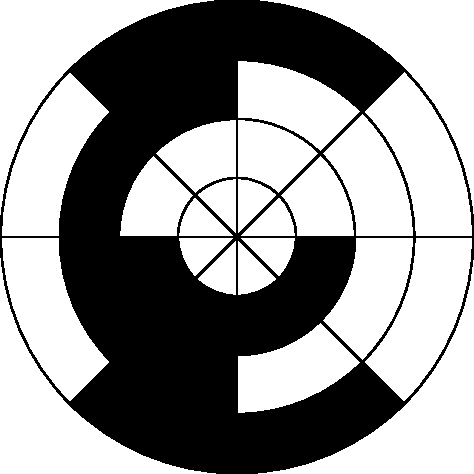
\includegraphics[height=.26\textheight]{encoderdisc}\hspace{4mm}
  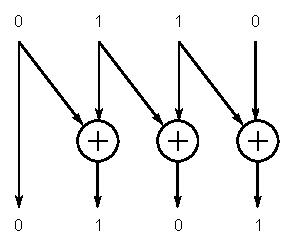
\includegraphics[height=.26\textheight]{bin2gray}\hspace{4mm}
  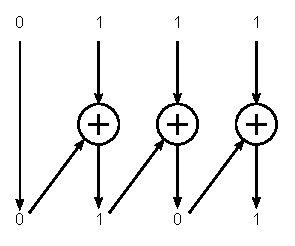
\includegraphics[height=.26\textheight]{gray2bin}\\[2mm]
  \begin{columns}[t]
  \begin{column}{.5\textwidth}
    \begin{block}{$0110_2$ to Gray}
      \small
      $g_0 = 0 \oplus 1 = 1$, $g_1 = 1 \oplus 1 = 0$,\\
      $g_2 = 1 \oplus 0 = 1$, $g_3 = 0$\\
      $\Rightarrow 0101_{\mathrm{Gray}}$
    \end{block}
  \end{column}
  \begin{column}{.48\textwidth}
    \begin{block}{$0110_{\mathrm{Gray}}$ to binary}
      \small
      $b_3 = 0$, $b_2 = 0 \oplus 1 = 1$,\\
      $b_1 = 1 \oplus 1 = 0$, $b_0 = 0 \oplus 0 = 0$\\
      $\Rightarrow 0100_2$
    \end{block}
  \end{column}
  \end{columns}
\end{frame}

\begin{frame}{ASCII and Unicode}
  \begin{columns}[t]
  \begin{column}{.5\textwidth}
    \begin{block}{ASCII}
      \small
      \begin{itemize}\itemsep1pt
        \item 7-bit code, 128 characters.
        \item First 32 codes are control codes; the rest are printable.
      \end{itemize}
      Example: `C' is column 100, row 0011, so $1000011_2 = 43_{16}$.
    \end{block}
  \end{column}
  \begin{column}{.48\textwidth}
    \begin{block}{Unicode}
      \small
      \begin{itemize}\itemsep1pt
        \item Covers Latin, Cyrillic, Arabic, Chinese, Japanese and emoji.
        \item Compatible with ASCII for the first 128 code points.
        \item Typically encoded as UTF-8.
      \end{itemize}
    \end{block}
  \end{column}
  \end{columns}
\end{frame}

\begin{frame}{Error Detection: Parity}
  \begin{columns}[t]
  \begin{column}{.5\textwidth}
    \begin{itemize}\small\itemsep2pt
      \item \alert{Even parity}: total number of 1s is even.
      \item Parity bit $p = b_3 \oplus b_2 \oplus b_1 \oplus b_0$.
      \item A single flipped bit gives odd parity: error detected.
      \item An even number of flipped bits is \alert{not} detected.
      \item Memory with SECDED can also \emph{correct} single-bit errors.
    \end{itemize}
  \end{column}
  \begin{column}{.48\textwidth}
    \centering\footnotesize\striped
    \begin{tabular}{@{}ccc@{}}
      \toprule
      \textbf{Char} & \textbf{ASCII} & \textbf{With even parity} \\
      \midrule
      S & 0110101 & 00110101 \\
      a & 1100001 & 11100001 \\
      l & 1101100 & 01101100 \\
      m & 1101101 & 11101101 \\
      ! & 0100001 & 00100001 \\
      \bottomrule
    \end{tabular}\\[1mm]
    {\scriptsize The unused MSB of each byte carries the parity bit.}
  \end{column}
  \end{columns}
\end{frame}

%===============================================================================
\section{Summary}
%===============================================================================

\begin{frame}{Summary}
  \begin{itemize}\itemsep3pt\small
    \item Every number system is positional: the weight of digit $i$ is $r^i$.
    \item Binary is native to hardware; octal and hex group 3 or 4 bits per character.
    \item Decimal to binary: repeated division by 2 (integers), repeated multiplication by 2 (fractions).
    \item \alert{BCD} stores each decimal digit in 4 bits: easy for humans, wasteful and needs special arithmetic.
    \item \alert{Gray code} changes one bit between consecutive values: rotary encoders, asynchronous crossings.
    \item \alert{ASCII} is the 7-bit baseline; Unicode (usually UTF-8) extends it.
    \item A parity bit detects any odd number of bit errors.
  \end{itemize}
  \begin{block}{Looking ahead}
    Chapter 3 extends these ideas to \emph{signed} numbers (sign--magnitude, one's and two's complement) and binary arithmetic.
  \end{block}
\end{frame}

\end{document}
